%% LyX 2.1.4 created this file.  For more info, see http://www.lyx.org/.
%% Do not edit unless you really know what you are doing.
\documentclass[english]{article}
\usepackage[T1]{fontenc}
\usepackage[latin9]{inputenc}
\usepackage{geometry}
\geometry{verbose,tmargin=2cm,bmargin=3cm,lmargin=1.5cm,rmargin=1.5cm}
\usepackage{float}
\usepackage{mathtools}
\usepackage{amsmath}
\usepackage{amssymb}
\usepackage{graphicx}
\usepackage{tablefootnote}
\usepackage{float}

\makeatletter

%%%%%%%%%%%%%%%%%%%%%%%%%%%%%% LyX specific LaTeX commands.
%% Because html converters don't know tabularnewline
\providecommand{\tabularnewline}{\\}
\floatstyle{ruled}
\newfloat{algorithm}{tbp}{loa}
\providecommand{\algorithmname}{Algorithm}
\floatname{algorithm}{\protect\algorithmname}

%%%%%%%%%%%%%%%%%%%%%%%%%%%%%% User specified LaTeX commands.
\usepackage{tikz}
\usepackage{babel}
\renewcommand{\labelitemi}{$\diamond$}
\newcommand{\T}{\rule{0pt}{2.6ex}}       % Top strut
\newcommand{\B}{\rule[-1.2ex]{0pt}{0pt}} % Bottom strut
\renewcommand{\vec}[1]{\boldsymbol{\mathbf{#1}}} % Vectors
\newcommand{\mat}[1]{\boldsymbol{\mathbf{#1}}} % Matrices
\usepackage{algorithm,algpseudocode}

\makeatother

\usepackage{babel}
\begin{document}

\title{COMP8620: MC-AIXI-CTW\\
Group 3}


\author{Jarryd Martin, John Aslanides, Yadunandan Sannappa,\\
 Nrupendra Rao, Cheng Yu, Ryk Budzynski}


\date{October 2015}

\maketitle
We outline an implementation of Veness et al.'s Monte Carlo AIXI approximation\cite{veness-11}
(MC-AIXI-CTW), and report our simulation results on a number of toy
domains.


\section{Introduction}

Recall that the AIXI agent is defined by its actions, which for each
cycle $k$ are given by 
\[
a_{k}^{\text{AIXI}}=\arg\max_{a_{k}}\sum_{o_{k}r_{k}}\cdots\max_{a_{m}}\sum_{o_{m}r_{m}}\left[r_{k}+\dots+r_{m}\right]\xi\left(o_{1}r_{1}\dots o_{m}r_{m}|a_{1}\dots a_{m}\right),
\]


where the $o_{n}$ and $r_{n}$ are the observation and reward provided
by the environment at cycle $n$, and $\xi$ is a Bayesian mixture
model for the environment. 

Following Veness et al., we approximate $a_{k}^{\text{AIXI}}$ using
Monte Carlo tree search (upper confidence bound) to approximate the
expectimax, and we compute a mixture over variable-order Markov models
using the context-tree weighting algorithm. 

We present a lightweight C++ implementation of MC-AIXI-CTW, along
with implementations of a number of simple games: $\textsc{Pacman},\ $
$\textsc{Tic-Tac-Toe}$, $\textsc{Biased Rock-Paper-Scissor}$, $\textsc{Extended-Tiger}$,
and $\textsc{Cheesemaze}$.


\section{User Manual}

To build from source, run ${\tt g++\ *.cpp\ *.hpp\ -o\ aixi}$ \textbf{TODO
check}

To run, invoke ${\tt ./aixi\ envname}$. 


\section{MC-AIXI-CTW Implementation}


\subsection{Main loop}

For each agent-environment interaction cycle, we run the following
for each experiment:

\begin{algorithm}
\begin{algorithmic}[1]
\renewcommand{\algorithmicrequire}{\textbf{Inputs:}}
\renewcommand{\algorithmicensure}{\textbf{Outputs:}}
\While{$cycle < max\_cycles$}
\While{environment is not finished}
\State{generate $(o,r)$ from environment}
\State{update agent model with $(o,r)$}
\If{explore}
\State{$a \leftarrow randomAction()$}
\Else
\State{$a \leftarrow MCTS()$}
\Comment{Monte Carlo Tree Search}
\EndIf
\State{perform action $a$}
\State{update agent history with $a$}
\State{$cycle++$}
\EndWhile
\State{reset environment}
\EndWhile
\end{algorithmic}

\caption{Main loop.}


\end{algorithm}


The $MCTS$ algorithm follows as in Algorithms 1-4 in Veness et al.,
and is found in ${\tt search.cpp}$. Model updates are handled in
methods in ${\tt agent.cpp}$, which interfaces with the context tree
defined in ${\tt predict.cpp}$.


\subsection{Monte Carlo Tree Search (MCTS) Algorithm}


\subsubsection{High level description}

Since the environment is only partially observable, we have no explicit
notion of state; instead, we only have a history of actions and percepts
$h=\left(a_{1}o_{1}r_{1}\dots a_{n}o_{n}r_{n}\right)$. For the purposes
of choosing the optimal action, we treat each possible (hypothetical)
history as a node in the search tree, with the root being the tip
of the current (realised) history. \\

The search tree is comprised of alternate layers of decision nodes and
chance nodes with the root being a decision node. The maximum branching
possible from decision nodes is the number of available actions in the given
environment while the maximum branching possible from chance nodes is equal
to the number of possible observations times the number of possible rewards.
We do however restrict branching in general to $100$ to avoid memory issues.
This number is configurable in ${\tt search.cpp}$. \\

Each node is implicitly labelled by its history as chance nodes record the
hypothetical action taken while decision nodes record the hypothetical
observation and reward from the environment.
The expected value of each node in the search tree is equal to the
expected total (non-discounted) reward that would be accumulated from
that node, where the expectation is under the agent's current policy
and the agent's current model for the behavior of the environment. \\

Thus, for each node we keep a value estimate $\hat{V}$, and a count
of the number of times $T$ that node has been visited in search.
This is used to determine how we explore the search space using the
UCB algorithm, which, for each decision node picks (assuming $T\left(ha\right)>0$
for all actions)
\[
a_{\text{UCB}}=\arg\max_{a\in\mathcal{A}}\left\{ \frac{1}{m\left(\beta-\alpha\right)}\hat{V}\left(ha\right)+C\sqrt{\frac{\log T\left(h\right)}{T\left(ha\right)}}\right\} ,
\]

where $\mathcal{A}$ is the set of all permissible actions, $m$ is
the search horizon, $\beta-\alpha$ is the difference between the
minimal and maximal instantaneous reward, and $C$ is a parameter
controlling the propensity of the agent to explore less frequently-seen
histories. \\

Note that the expectimax is a stochastic, partially observable game
between the agent and its environment. In the following, call nodes
corresponding to agent moves `decision nodes', and nodes corresponding
to Nature's moves `chance nodes'. \\

\subsubsection{Class structure}

To represent our search nodes, we define a base ${\tt SearchNode}$
class, from which ChanceNode and DecisionNode inherit. ChanceNode
and DecisionNode each have a ${\tt sample}$ method defined on them;
each of these methods is mutually recursive. For a given node $n$,
we keep its children in a dictionary keyed on the action or (observation,reward)
used to generate each child.

\subsubsection{Other Considerations}

In addition to the psuedocode presented in Veness et al., we implemented a solution
to allow us to decide on a per cycle basis whether or not to build a search tree from
scratch. In addition, we constructed routines which given an action taken by the
agent and an observation/reward received from the environment, would prune the search
tree accordingly. \\

The pruning of the search tree removes all subtrees begining with the chance nodes
directly below the root which correspond to the actions not taken by the agent and
as such are impossible future paths. Additionally, all subtrees begining with descision
nodes below the chance node (corresponding to the action taken) that do not match the
observation/reward received from the environment are pruned. As cycles progress
throughout an experiment, this represents a significant reduction in memory consumption. \\

Our final solution however did not implement pruning as our experimental results showed
unusual behaviour whereby the agent would appear to get stuck in certain game states.

\subsubsection{Efficiency/performance}

Between calls to ${\tt search}$, we retain much of the search tree,
pruning those nodes that are now inaccessible from the realised $(a,o,r)$
tuple that happened during the cycle. This allows us to avoid re-generating
similar search trees from similar positions. 


\subsection{Context Tree Weighting (CTW)}


\subsubsection{High level description of algorithm}


\subsubsection{Class structure}


\subsubsection{Code snippets}


\subsubsection{Efficiency/performance}


\section{Environments}
To test the effectiveness of the agent we developed 5 environment simulations which range in complexity from the relatively simple cheese maze to the much more complicated partially observable pacman game. The details of these environments with respect to their behaviour and implementation is discussed below. For all environments to avoid negative rewards to the agent we have added a constant to all rewards such that the minimum reward received by the agent is 0. Since the difference between the rewards is the same this will not affect the behaviour of the agent in any way.
\subsection{Cheese Maze}
This is a environment in which the agent is a mouse trying to find a piece of cheese in an two dimensional maze. The actions of the agent are:
\begin{center}
	\begin{tabular}{c | c}
		\textbf{Action} & \textbf{Code} \\
		\hline
		Move Up & 0 \\
		Move Right & 1 \\
		Move Left & 2 \\
		Move Down & 3 \\
		\hline
	\end{tabular}
\end{center}
The rewards have been adjusted as
\begin{center}
	\begin{tabular}{c | c}
		\textbf{Action effect} & \textbf{Reward} \\ \hline
		Agent bumps into wall & 0 \\
		Agent moves into free cell & 9 \\
		Agent finds cheese & 20 \\ \hline	
	\end{tabular}
\end{center}

\par
The details of the maze and the starting positions of the agent and the cheese are read from the configuration file. The maze is represented as the list of nodes as they would be visited by the depth first search algorithm. Mouse position and cheese position are simply the order of the node.\\
Each node of the maze is a structure which stores the percept of that node and an array of pointers which point to its neighbours. In case there is a wall on a particular side of the node then that pointer will be NULL. \\

In terms of an optimal agent strategy, an upper bound on reward per cycle for Cheesemaze is $2$ given that the best possible reward for an episode is $8$ and there are a minimum of $4$ moves (including the start) to reach the goal state.

\subsection{Extended Tiger}
This environment simulates two doors. At the start of each game the tiger is behind one of the doors with probability of 0.5 and behind the other door, there is a pot of gold. The agent begins sitting down and it can perform the following actions:
\begin{center}
	\begin{tabular}{c | c}
		\textbf{Action} & \textbf{Code} \\ \hline
		Stand & 0 \\
		Listen & 1 \\
		Open left door & 2 \\
		Open right door & 3 \\ \hline	
	\end{tabular}
\end{center}
When the agent tries to listen the environment provides it with an observation which correctly describes where the tiger is with a probability as defined in the configuration file. Until the listen action is performed the observation remains 0.
\begin{center}
	\begin{tabular}{c | c}
		\textbf{Observation} & \textbf{Code} \\ \hline
		Agent has not performed listen action yes & 0 \\
		Tiger behind left door & 1 \\
		Tiger behind right door & 2 \\ \hline
	\end{tabular}
\end{center}
The rewards the agent receives in this environment are as follows
\begin{center}
\begin{tabular}{c | c | c}
	\textbf{State} & \textbf{Action} & \textbf{Reward} \\ \hline
	sitting & stand & 99 \\
	sitting & open door & 90 \\
	sitting & listen & 99 \\
	standing & stand & 90 \\
	standing & open door with tiger & 0 \\
	standing & open door with gold & 30 \\
	standing & listen & 90 \\ \hline
\end{tabular}
\end{center}

In terms of an optimal agent strategy, an upper bound on reward per cycle for Extended Tiger is derived as follows. Firstly note that an optimal strategy will be to $\tt{start}$, $\tt{listen}$ $n$ times, $\tt{stand}$, $\tt{open}$. Letting a false observation probability be $q$, we wish to maximise the following w.r.t. $n$
$$\mathbb{E}[r_{\text{avg}}] = \frac{30(1-q)^n - 100(1-(1-q)^n)-n-1}{n+3}$$
where the denominator is equal to the number of actions taken. For example, with $q=0.15$, the optimal $n$ is $2$.

\subsection{Tic-Tac-Toe}
In this game, the agent plays games of TicTacToe against an opponent who makes random moves. The agent moves are coded as 0-8 referring to the different positions of the board.
\begin{center}
	\begin{tabular}{c | c | c}
	0 & 1 & 2 \\ \hline
	3 & 4 & 5 \\ \hline
	6 & 7 & 8 \\	
	\end{tabular}
\end{center}
Observation completely describes the current state of the board using 2 bits for each cell of the board. 
\begin{center}
	\begin{tabular}{c | l}
	00 & Cell empty \\
	01 & Agent's cell \\
	02 & Environment's cell \\
	\end{tabular}
\end{center}
The agent rewards are as follows:
\begin{center}
	\begin{tabular}{c | c}
	\textbf{Status} & \textbf{Reward} \\ \hline
	Illegal move & 0 \\
	Game is a draw & 4 \\
	Game won by agent & 5 \\
	Agent lost & 1 \\
	\end{tabular}
\end{center}

In terms of an optimal agent strategy, an upper bound on reward per cycle is $0.5$ given that the minimu number of cycles required for the agent to win the game is $4$.

\subsection{Biased Rock-Paper-Scissors}
The agent will play games of Rock-Paper-Scissors against an opponent who plays the same action every time it wins the game, and otherwise plays a random move. For this agent we encoded the actions of the agent and the environment as
\begin{center}
	\begin{tabular}{c | c}
	Rock & 0 \\
	Paper & 1 \\
	Scissors & 2 \\
	\end{tabular}
\end{center}
The agent receives a reward of 1 for a win, 0 for a draw and -1 for a loss. \\

In terms of an optimal agent strategy, an upper bound on reward per cycle for Biased Rock-Paper-Scissors is derived as follows.

Let $X_t$ be a R.V. representing the outcome of cycle $t$. Under an optimal strategy, the agent will win after the environment won in cycle $t-1$ as the environments action in cycle $t$ is predictable. Otherwise, the agent plays randomly. As such we have
$$P(X_t = \text{win}) = \sum_{X_{t-1}} P(X_t = \text{win}, X_{t-1}) = \sum_{X_{t-1}} P(X_t = \text{win}|X_{t-1})P(X_{t-1})$$
which is a 1\textsuperscript{st} order Markov chain with the following right stochastic transition matrix

\begin{align}
\mat{P} = 
\begin{bmatrix}
\frac{1}{3} & \frac{1}{3} & \frac{1}{3} \\
1 & 0 & 0 \\
\frac{1}{3} & \frac{1}{3} & \frac{1}{3}
\end{bmatrix}
\end{align}

Therefore, we want a steady state distribution for $\mat{P}$, i.e. a solution to $\vec{\pi} = \mat{P}\vec{\pi}$, which is an eigenvector $\vec{\pi^{*}}$. The average reward at time $t$ is then
$$\mathbb{E}[r_{\text{avg}_t}] = 1 \cdot P(X_t = \text{win}) + 0 \cdot P(X_t =\text{draw}) - 1 \cdot P(X_t = \text{lose}) = \vec{\pi^{*}_0} - \vec{\pi^{*}_2} = 0.25$$

\subsection{PacMan}
This is game of PacMan in which the agent can only partially observe the environment unlike the classic game in which the entire game state is known to the player at any given time. The agent does not know the structure of the maze but only receives a 4 bit wall configuration of the node it is currently in. The agent also receives a 4 bit observation of the presence of any ghosts in its direct line of sight. The location of food pellets can change every episode as every free cell has a 50\% chance of having food in it. The agent receives a 3 bit observation indicating the presence of food within a Manhattan distance of 2, 3 or 4. It also receives a 4 bit string indicating food in its line of sight similar to the ghosts. The agent also knows when it is under the effect of the power pill.\\
\begin{center}
	\begin{tabular}{c | c}
	\textbf{Action} & \textbf{Reward} \\ \hline
	Agent runs into a wall & -10 \\
	Agent caught by a ghost & -50 \\
	Agent moves into empty cell & -1 \\
	Agent eats a food pellet & 10 \\
	Agent collects all the food & 100 \\
	\end{tabular}
\end{center}
To calculate the actual reward, the rewards from the above table are added to 60. This is because the agent can potentially be affected by multiple rewards e.g. it can run into a wall and get caught by a ghost in the same turn.

In terms of an optimal agent strategy, an upper bound on reward per cycle for Pacman is unknown.

\section{Simulation Results}

\subsection{Experiment Summary}
Following is a complete summary of all experiments conducted \\

\begin{table}[H]
\begin{tabular}{|l|l|l|l|l|l|l|l|l|}
\hline 
 & Bits\tablefootnote{total bit length of an $\tt{ora}$ cycle} & CT-depth & Cycles & Timeout\tablefootnote{timeout value for each select action} & Horizon & Exp. Rate & Exp.-Decay & UCB-weight\tablefootnote{UCB exploration bias parameter} \tabularnewline
\hline 
Cheesemaze & $11$ & $96$ & $10$ & $0.5$ & $8$ & $0.999$ & $0.999769818$ & $1.4$ \tabularnewline
           & $11$ & $96$ & $10$ & $1.6$ & $6$ & $0.999$ & $0.999769818$ & $1.4$ \tabularnewline
           & $11$ & $144$ & $2.5$ & $3$ & $8$ & $0.999$ & $0.9990795899$ & $1.4$ \tabularnewline
           & $11$ & $48$ & $10$ & $0.1$ & $4$ & $0.999$ & $0.999769818$ & $1.4$ \tabularnewline
           & $11$ & $96$ & $10$ & $0.5$ & $8$ & $0.999$ & $0.999769818$ & $1.4$ \tabularnewline
\hline
Biased Rock-Paper-Scissors & $6$ & $32$ & $10$ & $2.5$ & $4$ & $0.999$ & $0.999769818$ & $1.4$ \tabularnewline
                           & $6$ & $48$ & $5$ & $5$ & $8$ & $0.999$ & $0.999539689$ & $1.4$ \tabularnewline
                           & $6$ & $96$ & $4.5$ & $4$ & $4$ & $0.999$ & $0.9994885564$ & $1.4$ \tabularnewline
                           & $6$ & $96$ & $10$ & $0.5$ & $4$ & $0.999$ & $0.999$ & $1.4$ \tabularnewline
\hline
Extended Tiger & $13$ & $96$ & $16$ & $2.5$ & $6$ & $0.999$ & $0.99985613$ & $1.4$ \tabularnewline
               & $13$ & $96$ & $2.5$ & $12$ & $4$ & $0.999$ & $0.9990795899$ & $1.4$ \tabularnewline
               & $13$ & $96$ & $25$ & $0.8$ & $4$ & $0.999$ & $0.9999079208$ & $1.4$ \tabularnewline
               & $13$ & $52$ & $5$ & $8$ & $4$ & $0.999$ & $0.999539689$ & $1.4$ \tabularnewline
\hline
Tic-Tac-Toe    & $25$ & $96$ & $4.5$ & $4$ & $9$ & $0.9999$ & $0.9994884564$ & $1.4$ \tabularnewline
               & $25$ & $192$ & $5$ & $8$ & $9$ & $0.9999$ & $0.999539599$ & $1.4$ \tabularnewline
               & $25$ & $256$ & $20$ & $8$ & $9$ & $0.9999$ & $0.9998848799$ & $1.4$ \tabularnewline
               & $25$ & $512$ & $25$ & $3$ & $9$ & $0.9999$ & $0.9999079028$ & $1.4$ \tabularnewline
               & $25$ & $512$ & $30$ & $2$ & $9$ & $0.9999$ & $0.9999232518$ & $1.4$ \tabularnewline
\hline
Pacman         & $26$ & $256$ & $10$ & $4$ & $8$ & $0.99$ & $0.999$ & $1.5$ \tabularnewline
               & $26$ & $512$ & $20$ & $2$ & $4$ & $0.9999$ & $0.9998848799$ & $1.4$ \tabularnewline
               & $26$ & $320$ & $10$ & $4$ & $8$ & $0.99$ & $0.999$ & $1.4$ \tabularnewline
               & $26$ & $256$ & $10$ & $1$ & $6$ & $0.9999$ & $0.999769773$ & $1.4$ \tabularnewline
\hline 
\hline
\end{tabular}
\caption{MC-AIXI-CTW Experiments}
\end{table}

\subsection{Cheesemaze}
Here we present the environmental setup and learning rate of our best results
training AIXI on the Cheesemaze environment. \\

Interpreting the results, we conclude that ... \\

\begin{table}[H]
\centering
\begin{tabular}{|l|l|l|l|l|l|l|l|}
\hline 
Bits & CT-depth & Cycles & Timeout & Horizon & Exp. Rate & Exp.-Decay & UCB-weight \tabularnewline
\hline 
$11$ & $96$ & $10$ & $0.5$ & $8$ & $0.999$ & $0.999769818$ & $1.4$ \tabularnewline
\hline
\end{tabular}
\caption{Environment Setup}
\end{table}

\begin{figure}[h!]
\centering
\caption{Learning Rate}
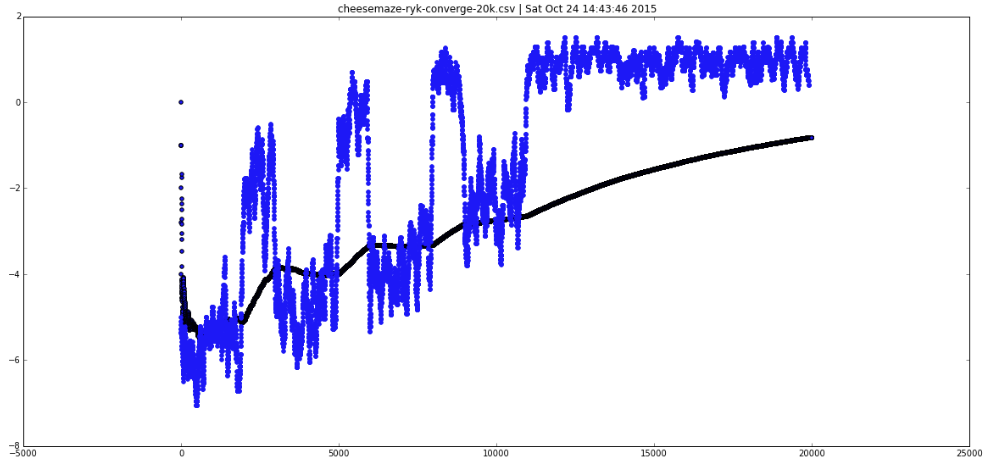
\includegraphics[scale=0.4]{cheesemaze_best} 
\end{figure}

\subsection{Extended Tiger}
Here we present the environmental setup and learning rate of our best results
training AIXI on the Extended Tiger environment. \\

Interpreting the results, we conclude that ... \\

\begin{table}[H]
\centering
\begin{tabular}{|l|l|l|l|l|l|l|l|}
\hline 
Bits & CT-depth & Cycles & Timeout & Horizon & Exp. Rate & Exp.-Decay & UCB-weight \tabularnewline
\hline 
$11$ & $96$ & $10$ & $0.5$ & $8$ & $0.999$ & $0.999769818$ & $1.4$ \tabularnewline
\hline
\end{tabular}
\caption{Environment Setup}
\end{table}

\begin{figure}[H]
\centering
\caption{Learning Rate}
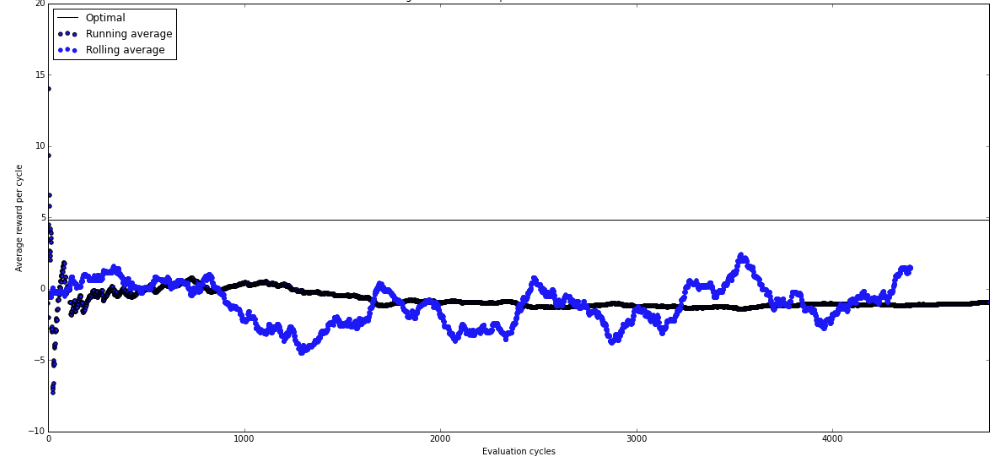
\includegraphics[scale=0.4]{tiger_best} 
\end{figure}

\subsection{Tic\-Tac\-Toe}
Here we present the environmental setup and learning rate of our best results
training AIXI on the Tic-Tac-Toe environment. \\

Interpreting the results, we conclude that ... \\

\begin{table}[H]
\centering
\begin{tabular}{|l|l|l|l|l|l|l|l|}
\hline 
Bits & CT-depth & Cycles & Timeout & Horizon & Exp. Rate & Exp.-Decay & UCB-weight \tabularnewline
\hline 
$11$ & $96$ & $10$ & $0.5$ & $8$ & $0.999$ & $0.999769818$ & $1.4$ \tabularnewline
\hline
\end{tabular}
\caption{Environment Setup}
\end{table}

\begin{figure}[H]
\centering
\caption{Learning Rate}
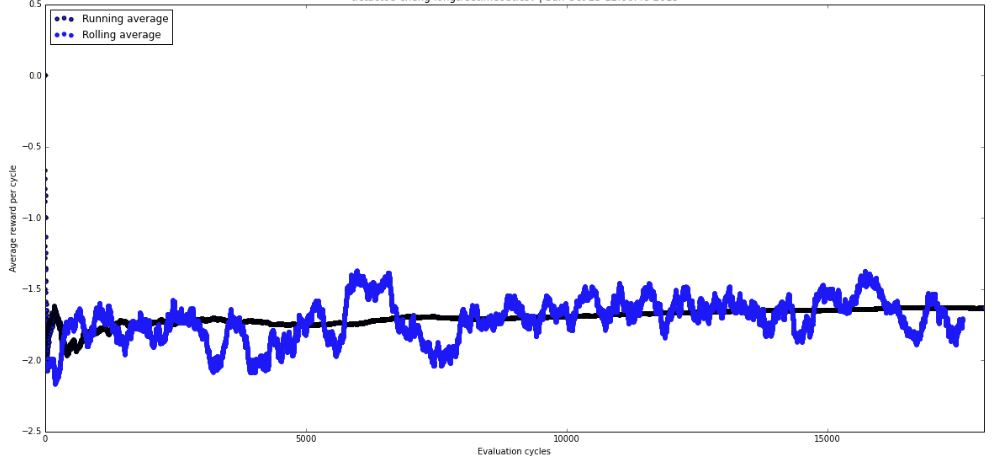
\includegraphics[scale=0.4]{tictactoe_best} 
\end{figure}

\subsection{Biased Rock-Paper-Scissors}
Here we present the environmental setup and learning rate of our best results
training AIXI on the Biased Rock-Paper-Scissors environment. \\

Interpreting the results, we conclude that ... \\

\begin{table}[H]
\centering
\begin{tabular}{|l|l|l|l|l|l|l|l|}
\hline 
Bits & CT-depth & Cycles & Timeout & Horizon & Exp. Rate & Exp.-Decay & UCB-weight \tabularnewline
\hline 
$11$ & $96$ & $10$ & $0.5$ & $8$ & $0.999$ & $0.999769818$ & $1.4$ \tabularnewline
\hline
\end{tabular}
\caption{Environment Setup}
\end{table}

\begin{figure}[H]
\centering
\caption{Learning Rate}
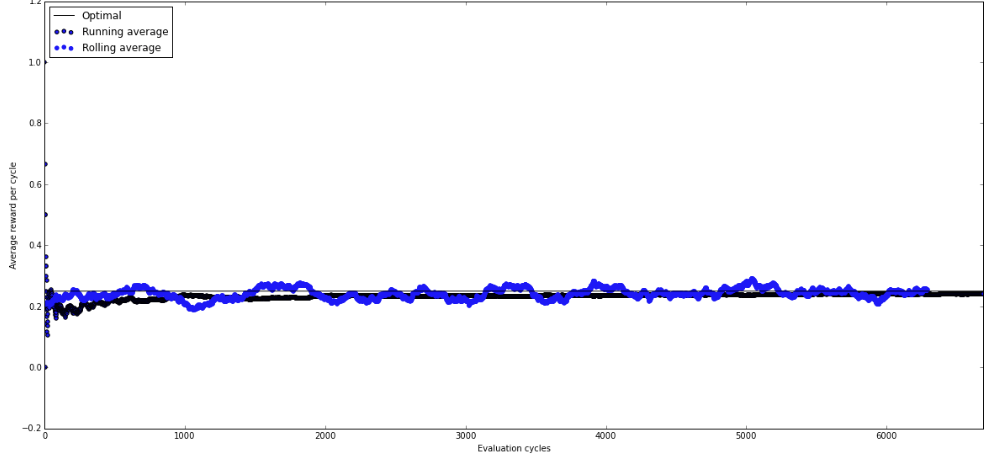
\includegraphics[scale=0.4]{rockpaper_best} 
\end{figure}

\subsection{Pacman}
Here we present the environmental setup and learning rate of our best results
training AIXI on the Pacman environment. \\

Interpreting the results, we conclude that ... \\

\begin{table}[H]
\centering
\begin{tabular}{|l|l|l|l|l|l|l|l|}
\hline 
Bits & CT-depth & Cycles & Timeout & Horizon & Exp. Rate & Exp.-Decay & UCB-weight \tabularnewline
\hline 
$11$ & $96$ & $10$ & $0.5$ & $8$ & $0.999$ & $0.999769818$ & $1.4$ \tabularnewline
\hline
\end{tabular}
\caption{Environment Setup}
\end{table}

\begin{figure}[H]
\centering
\caption{Learning Rate}
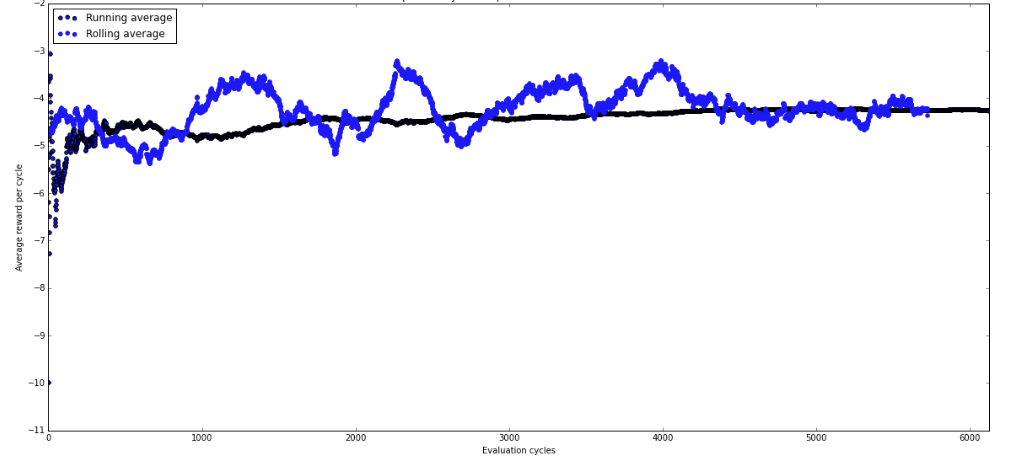
\includegraphics[scale=0.4]{pacman_best} 
\end{figure}

\section{Cross Domain Simulation Results}
\begin{itemize}
\item Cheesemaze and Extended Tiger
\item Cross domain simulation on more difficult environments... 
\item Separate CTW for Obs and Rews...
\end{itemize}

\section{Discussion and Conclusions}


\section*{Appendix}

\appendix

\section{Files}

The report archive should contain the following: 
\begin{verbatim}

MC-AIXI-CTW-Grp3.zip
    \report
        report.pdf // this report
        report.tex
        cheesemaze_best.png // results plots
        tiger_best.png
        rockpaper_best.png
        tictactoe_best.png
        pacman_best.png
    \src
        main.hpp
        main.cpp
        environment.hpp
        environment.cpp
        agent.hpp
        agent.cpp
        search.hpp
        search.cpp
        predict.hpp
        predict.cpp
        util.hpp
        util.cpp
        README.md
        cheesemaze.conf // environment configuration files
        rockpaper.conf
        tictactoe.conf
        coinflip.conf
        tiger.conf
\end{verbatim}

\section{Graphs..}

\bibliographystyle{unsrt}
\bibliography{report}

\end{document}
